\chapter{関連研究}
\label{chap:webapi}

本章ではユーザの仮想現実や明晰夢における認識度や要求について事前調査、睡眠に関する調査、睡眠中に見たい夢の分析を行った。そしてDreamDateの開発に反映した点について述べる。

\section{夢と睡眠}
睡眠中に扱うアプリケーションの開発にあたって、睡眠自体を理解することは不可欠である。関連研究の調査によって明らかになった睡眠段階や夢についてここで記す。

\subsection{夢と記憶}
夢は空間及び時間軸からすると、登場人物が非現実的な場合など不合理で異様な内容のことが多いが、大抵の場合人は、現実だと錯覚し夢を見ていることに気がつかない。それは論理的思考力を担う前頭前皮質の機能が低下しているためだ\cite{cortex}。起床後も夢での感情が現実で起きたかのように勘違いしてしまうほどリアルな体験をする人も多い。起床後すぐに夢日記をとれば、本当の思い出のように夢の記憶が残る場合もある。心理学者であるフロイト(Sigmund Freud)は1905年に無意識の欲求や感情、抑圧された子供の頃の記憶、生理的欲求などが夢に大きな影響を与えていると述べた\cite{freud}。一方で2006年にZhangは夢は短期的な記憶を長期的な記憶に変換するためのプロセスであると述べている。図\ref{brainZhang}は睡眠中の脳の記憶モデルである\cite{Zhang}。脳の容量には限度があるため、睡眠中に過去の記憶の中で関連性の強い記憶を繋げたり、重複している内容や必要のない記憶を消しているのだ\cite{Zhang}。睡眠時間が減ると暗記能力が減るのもこれにより説明できる。\\
 幼児の平均睡眠時間は16時間でそのう内の50\%をレム睡眠が占める。一方成人の平均睡眠時間は7時間でレム睡眠も短いため、夢をあまり見なくなる。年齢が若いほどレム睡眠の周期が長いのは、経験すること全てが新しいため多くのことを記憶しなければならないことと、脳の空き容量が多いためと説明されている\cite{Zhang}。

\begin{figure}[htbp]
\begin{center}
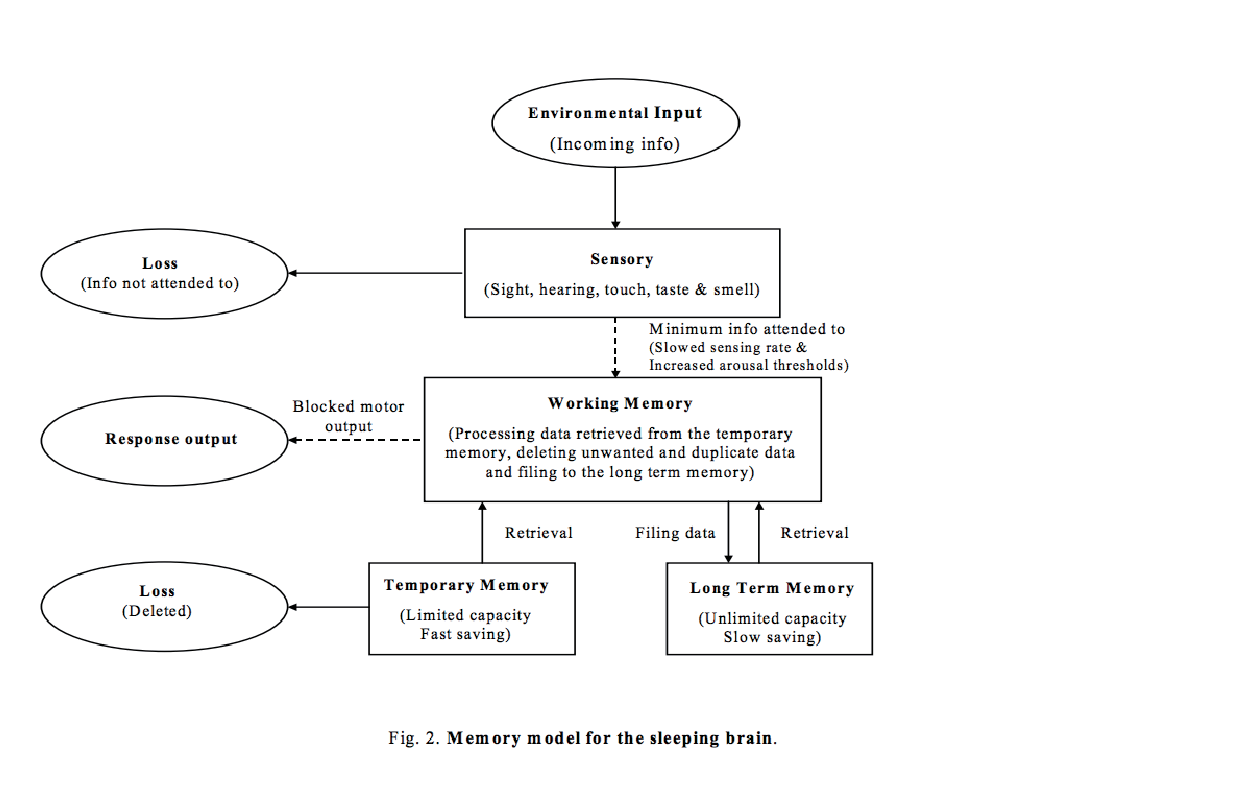
\includegraphics[width=13cm]{eps/sleepBrainModel.eps}
\caption{睡眠中の脳の記憶モデル(Zhang, 2006, p.3)}
\label{brainZhang}
\end{center}
\end{figure}

\subsection{睡眠と睡眠段階(睡眠の深さのレベル)}
 睡眠は身体を休めるためにある。人生の1/3を占める活動である。そして睡眠中人は2つの睡眠段階、レム睡眠とノンレム睡眠を90分間隔で行き来している\cite{Dement}。筑波大学と理化学研究所の研究によるとレム睡眠中は記憶形成や脳機能回復の作用がある脳波(デルタ波)が多く見られるというのが通説である\cite{tsukuba}。そしてレム睡眠中は心拍数や眼球の運動が活発化する。レム睡眠の最中に起きたときは夢も比較的覚えているという研究もされている\cite{remNonrem}。一方ノンレム睡眠中は脳も身体も休んでいる。\\
 図\ref{SleepHypnogram}は平均的な睡眠のサイクルを示したものである\cite{hypnogram}。睡眠に突入して初めてのレム睡眠は10〜12分でもっとも短い。2度目のレム睡眠は15〜20分。最後の夢は15分であるが、通常はアラームなどによって不意に中断されることが多い。平均的に一晩で5〜7回夢をみる。一般的な人生で人は6年間夢を見る。DreamDateはこの6年間をより充実感のある体験にするために貢献できるアプリケーションになる可能性がある。

\begin{figure}[htbp]
\begin{center}
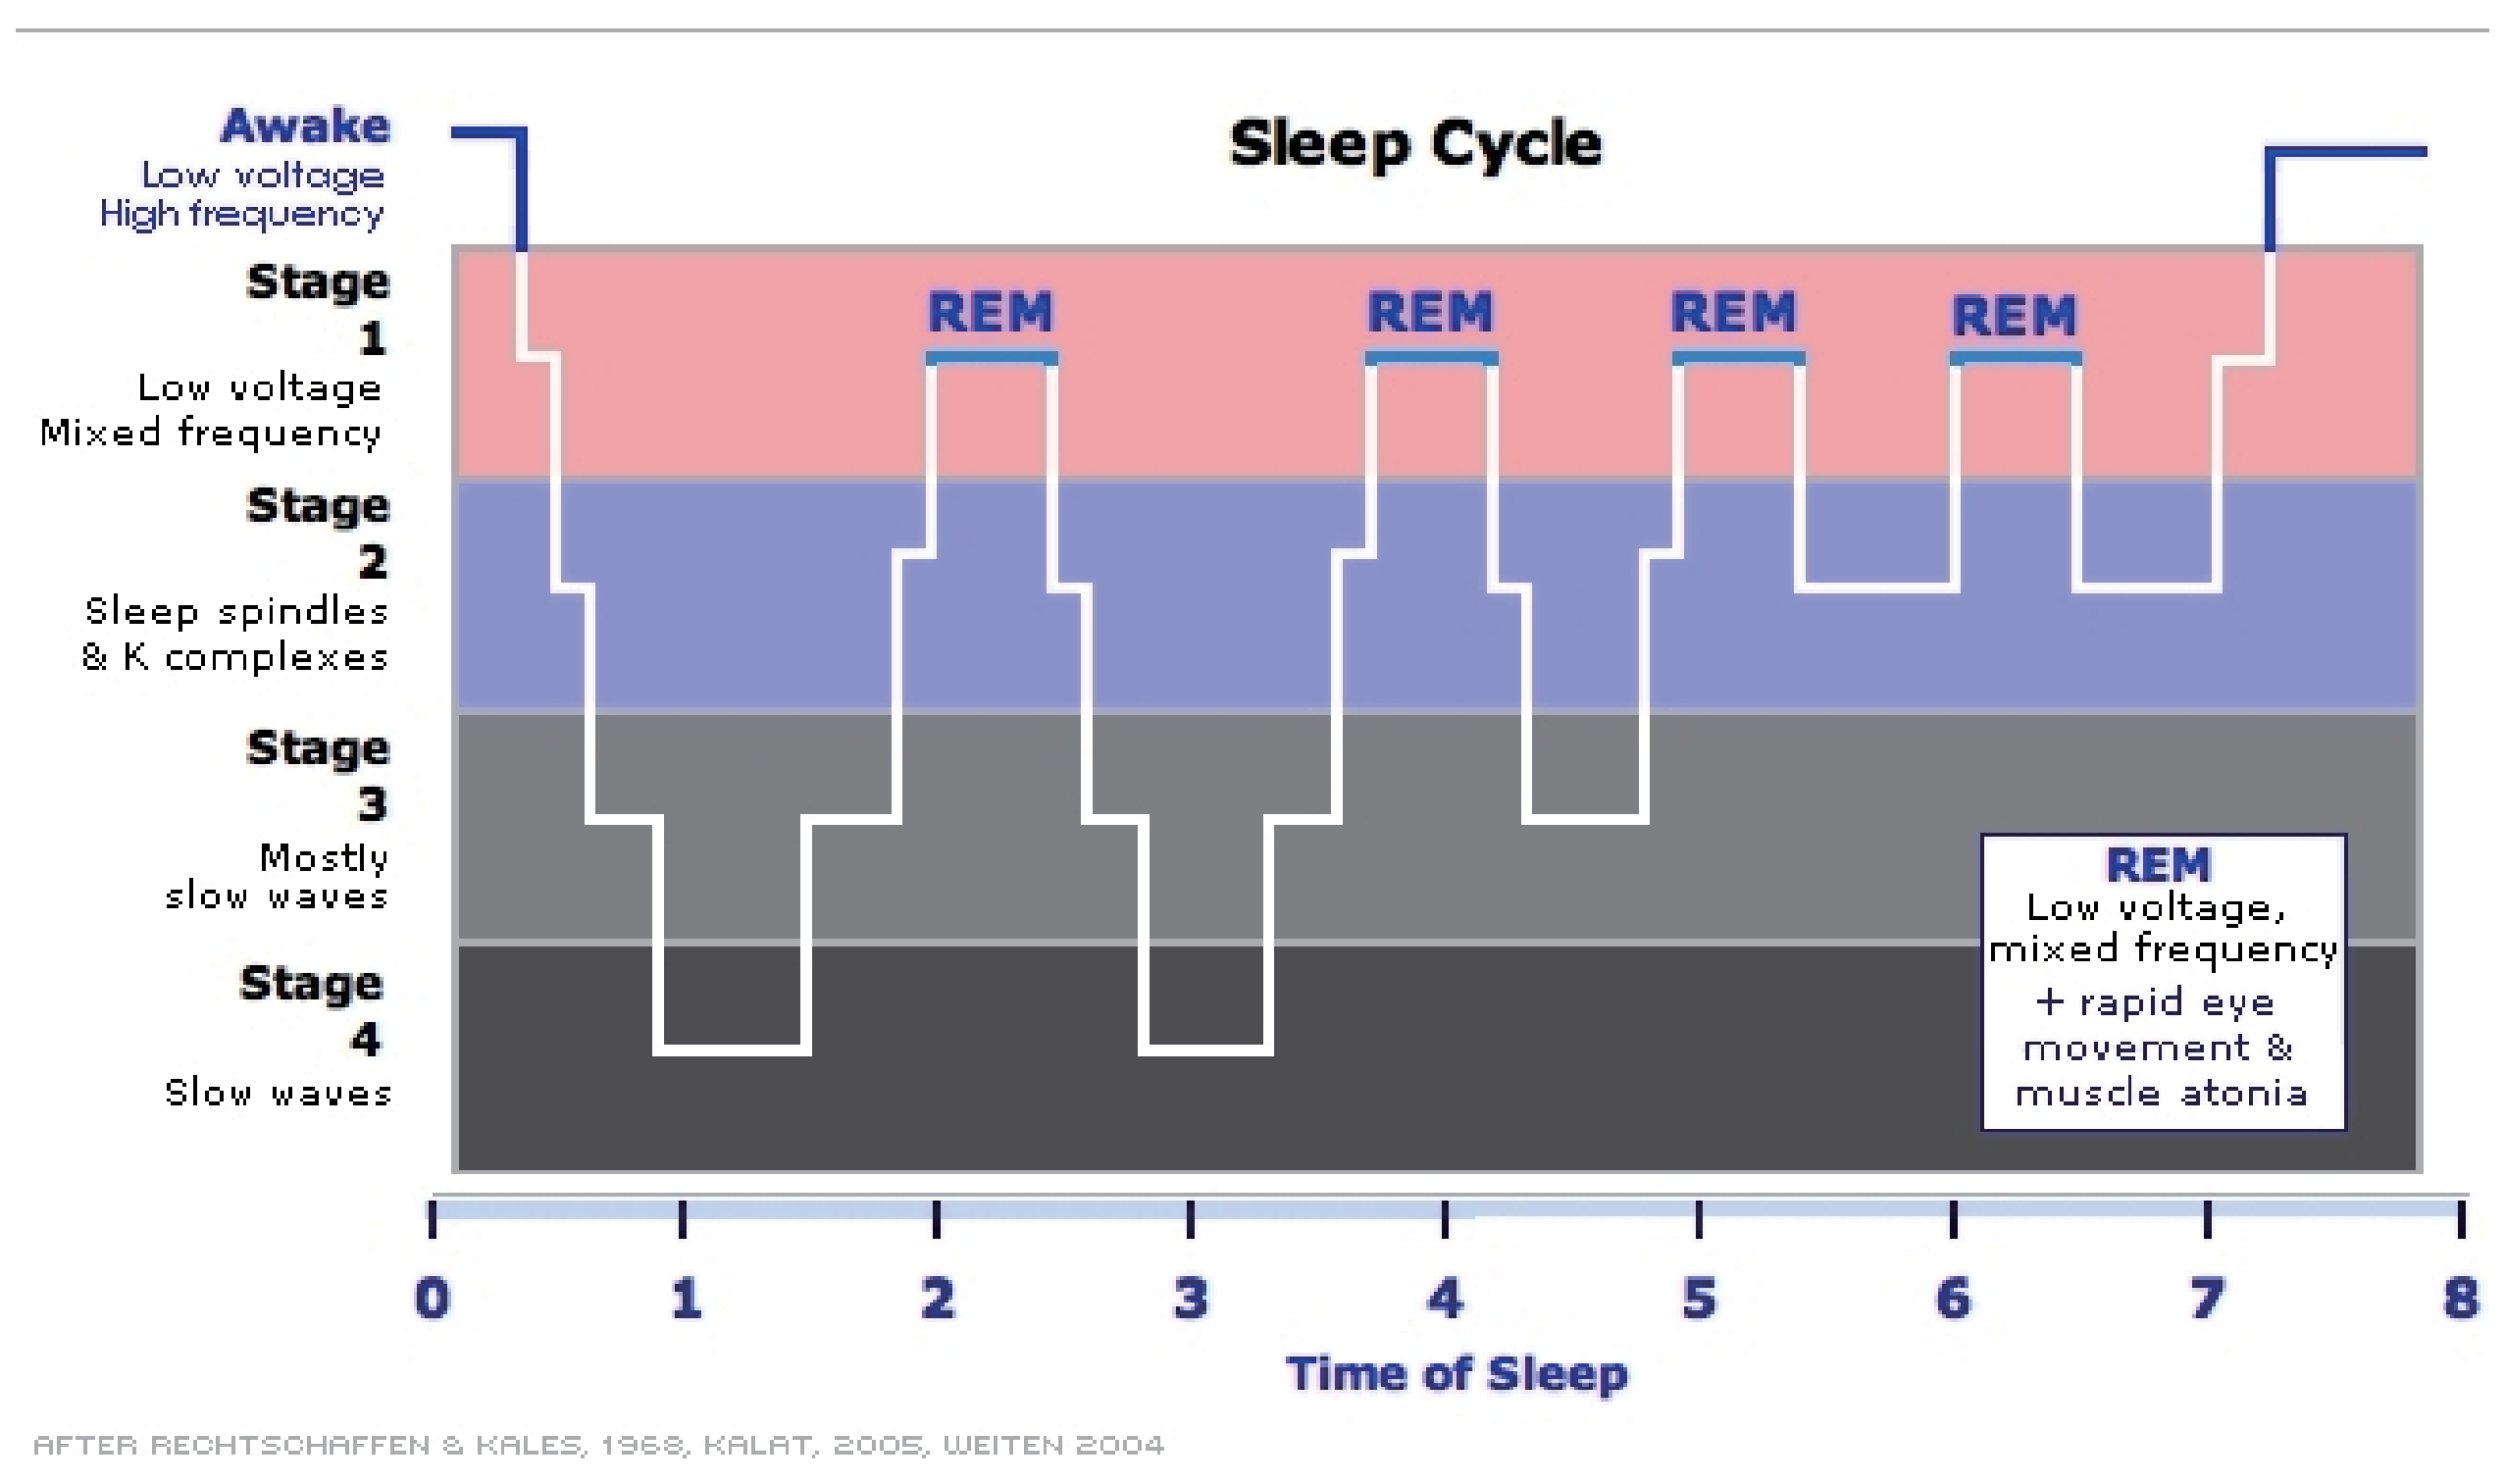
\includegraphics[width=15cm]{eps/SleepHypnogram.eps}
\caption{睡眠サイクルの図 (Catalyst Athletics, 2004, p.1) }
\label{SleepHypnogram}
\end{center}
\end{figure}

\subsection{睡眠段階のセンシング方法}
睡眠段階のセンシング方法として正確性が高いのは脳波センサーである。しかしそれ以外のセンシング方法もある。人はレム睡眠中に眼球が活発化し心拍数が多少上がるので、眼球の運動と心拍によりセンシングが可能である。人は睡眠段階を移行させるために寝返りを行う習性があるとされている。要するに睡眠サイクルのスイッチのような働きをする\cite{negaeri}。よって寝返りをモニタリングすれば睡眠段階をある程度センシングすることが可能であるということが通説となっている。

\section{明晰夢に関するアンケート調査}
彼に提案手法によって夢の操作に成功したとしてもその夢を覚えていなければ意味がない。そこでユーザスタディーを始める前に、一般的に人は夢の内容を起床後どのくらい覚えているのかを20〜60歳の男女27人にオンラインアンケートをした。夢をよく覚えていると答えた人は内容によっては覚えていると答えたのは10人、覚えていないとこ答えたのは13人、よく覚えているのと答えたのは4人であった。
%\begin{figure}[htbp]
%\begin{center}
%\includegraphics[width=15cm]{eps/レムember.eps}
%\caption{夢を覚えている比率}
%\label{レムemberDream}
%\end{center}
%\end{figure}

覚えている夢は刺激的、怖い夢、繰り返し見た夢というのが多く、日常的な夢は忘れがちであるということが分かった。人は睡眠中の夢の90\%を起床後5分間で忘れるという。Zhangによるとレム睡眠中は短期的な記憶を担っている脳は長期的な記憶への移行に注力していて、インプットの部分があまり機能していないためであると説明する\cite{Zhang}。ただ起きてすぐに夢日記で夢を記憶すれば覚えていられることも可能である\cite{forgetDreams}。\\
Freudは「夢判断」の中で人は睡眠中の姿勢、環境、身体的刺激によって夢の内容が変化すると述べた\cite{freud}。睡眠中の人間の鼻先を羽毛でくすぐったときに、夢の内容に変化があったことを確認する実験を紹介している。そこで音、体制、匂い、振動、光、などの刺激の中で何が夢に一番影響を与えやすいのかを男女27人にオンラインアンケートをとった。図\ref{externalShigeki}にその結果を示す。音が他の刺激よりも影響を与えやすいということが分かった。また学術的にも聴覚と嗅覚は人間の生命維持を高めるために感度は低いが睡眠中も機能しているということが証明されている\cite{Zhang}。\\

\begin{figure}[htbp]
\begin{center}
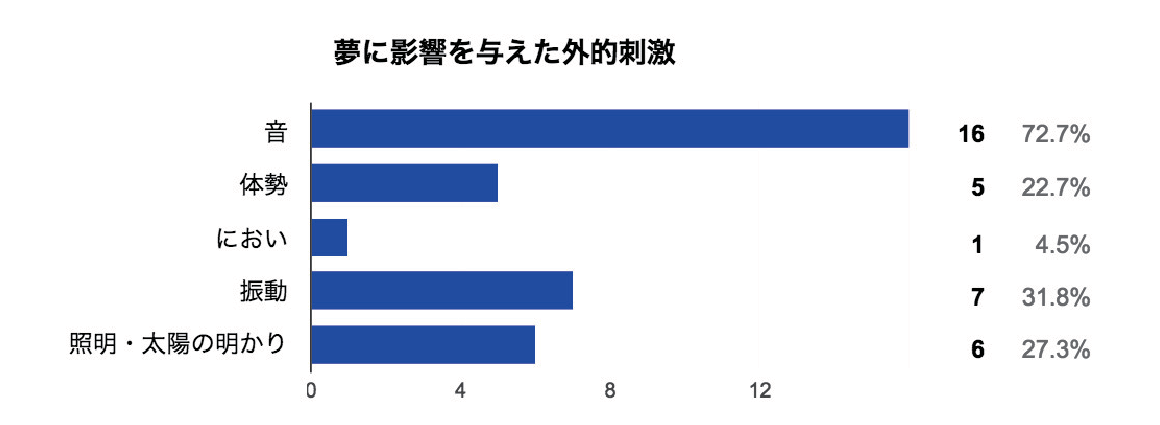
\includegraphics[width=15cm]{eps/input.eps}
\caption{夢に影響を与えた外的刺激}
\label{externalShigeki}
\end{center}
\end{figure}

明晰夢を体験したいか否かで質問をしたところ77\%の人が体験したいと答えた。図\ref{desiredDreamTpye}は仮想現実で体験したい内容を調査結果から似ているものをカテゴリー別に分けたものである。LOVEタイプ、癒しタイプ、元気欲しいタイプ、アドベンチャータイプ、ストーリータイプ、ビジネスタイプと分類を行った。LOVEタイプとは恋愛や性的行為などが含まれるもの、アドベンチャータイプは冒険など非日常の体験を求めるもの、ストリータイプはドラマのように連続性のある夢を求めるもの、癒しタイプ・元気欲しいタイプは娯楽を求めるもの、原強化タイプは睡眠中になんらかの学習を求める内容。LOVEタイプと癒し・元気が欲しいタイプが最も多く、少数派としてビジネスタイプである。\\

\begin{figure}[htbp]
\begin{center}
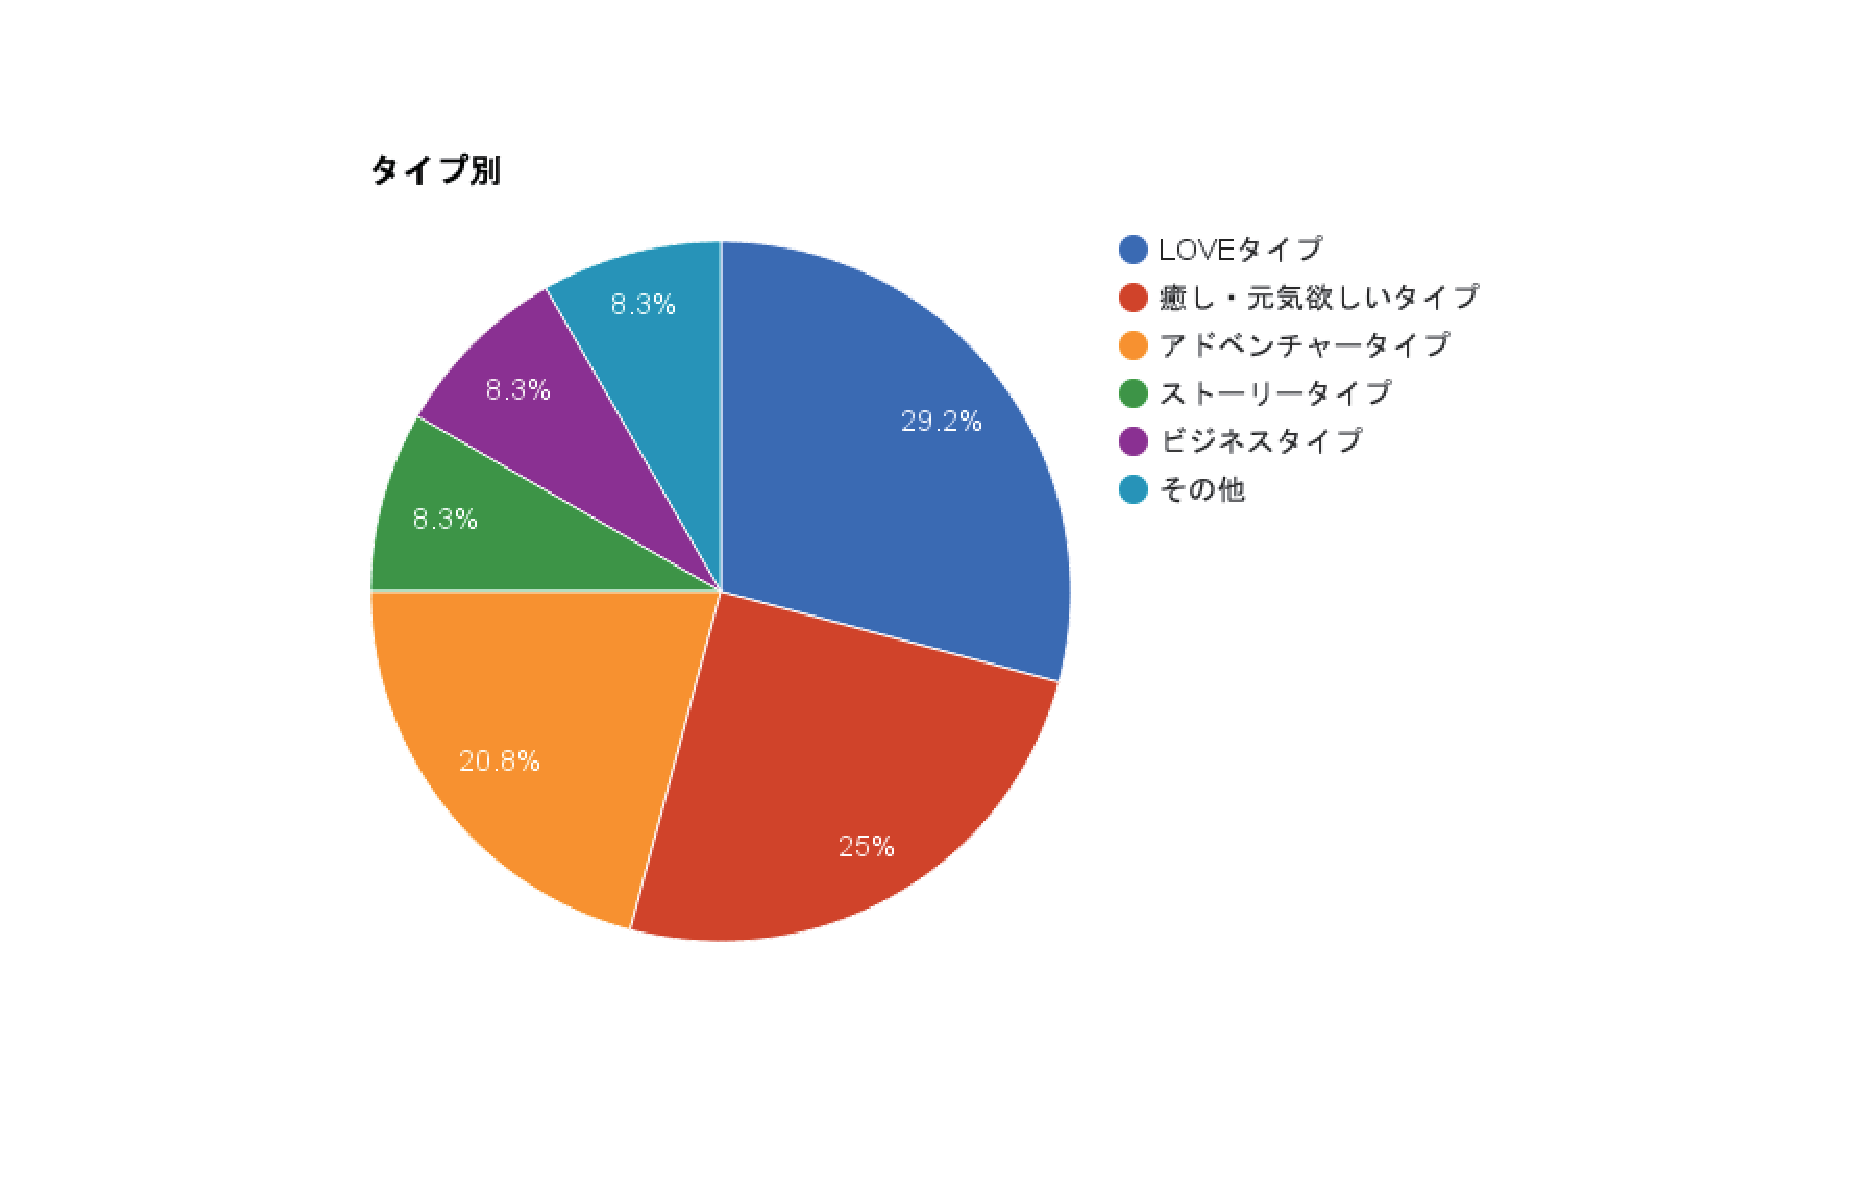
\includegraphics[width=15cm]{eps/dreamType.eps}
\caption{明晰夢で体験したい内容のカテゴリ:分析1}
\label{desiredDreamTpye}
\end{center}
\end{figure}

回答をさらに違った方法で分析した結果が\ref{desiredDreamTpye2}である。これらの結果からユーザによって理想の夢は日常や非日常、具体性や抽象性に隔たりがあり、一貫性が見られないことがわかった。

\begin{figure}[htbp]
\begin{center}
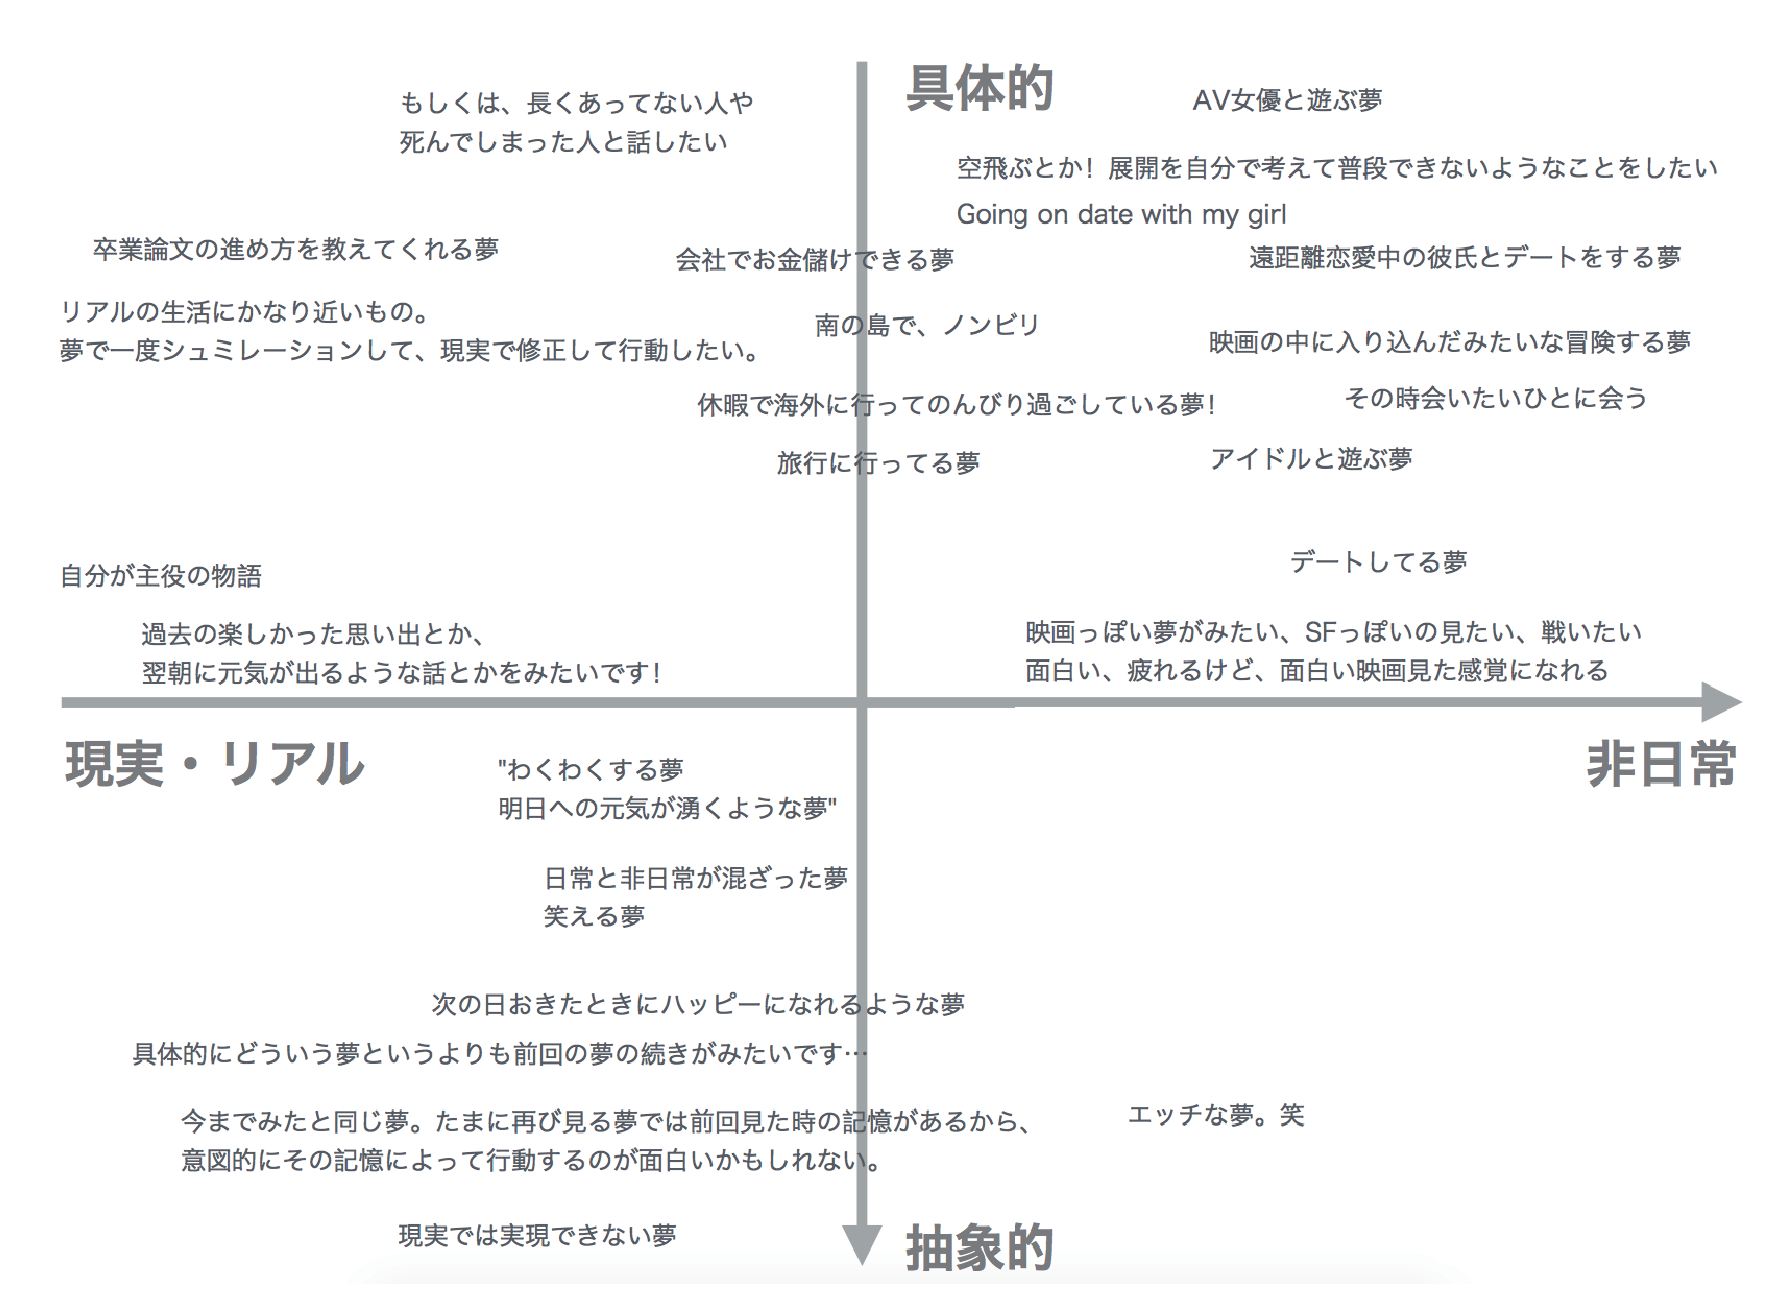
\includegraphics[width=13cm]{eps/whatYouWantToDream.eps}
\caption{明晰夢で体験したい内容の詳細:分析2}
\label{desiredDreamTpye2}
\end{center}
\end{figure}


\section{仮想現実システムに関するアンケート調査}
人々がどのような仮想現実を望んでいるかを調査するため20〜60歳の男女27人にGoogle Docのサーベイ機能を使ってオンラインアンケートをした。これらのインタビュー結果を経て一般的なユーザのニーズを把握し、DreamDateの有効性やDreamDateが解決すべき問題について明らかにする。

%\subsection{仮想現実を体験するために一般的な人々が支払う金額}
%各所公式ウェブサイトを掲載し、機能性やデザインの詳細を説明した上で、仮想現実を見る手段として次の選択肢から購入しようと思う商品を選んでもらった。

%\begin{itemize}
%\item OCULOUS Rift:85278円
%\item ハコスコ:1500円
%\item iWink:36478円
%\item タカラトミー夢見工房:15984円
%\item DreamDate :無料
%\end{itemize}

%すると図\ref{userNeedCost}のように、一般ユーザの中には仮想現実を体験するためにOCULOUS Riftなどの高額なデバイスを購入しようとする人は少ないということが分かった。1500円ハコスコだと少し数が増えるが、これらのデータから無料で簡単に手に入れることができるツールを多くの人が必要としていることが示唆された。

%\begin{figure}[htbp]
%\begin{center}
%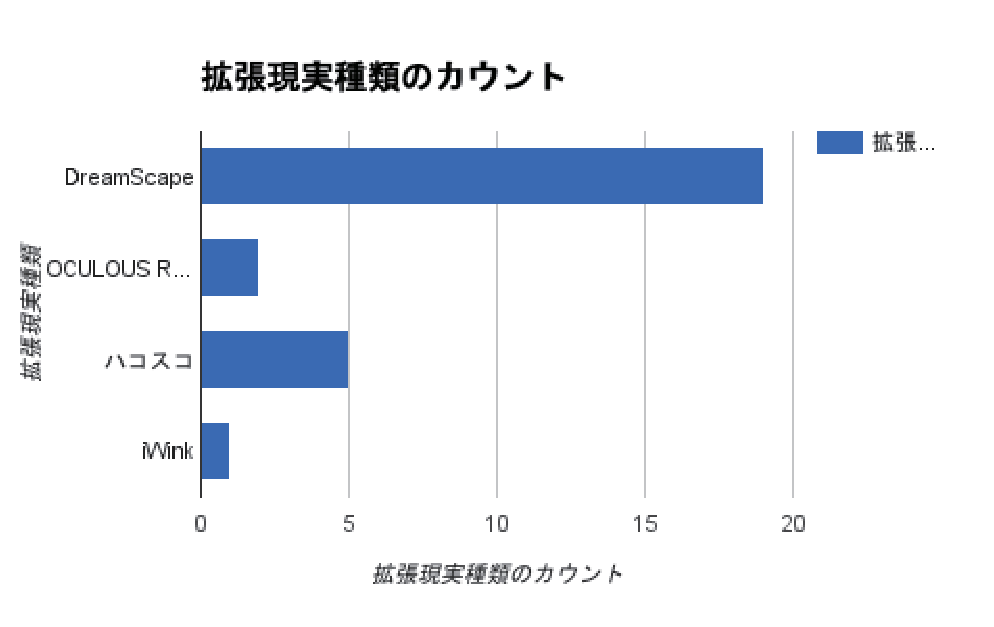
\includegraphics[width=15cm]{eps/VRselection.eps}
%\caption{仮想現実を体験するために一般的ユーザが選ぶデバイス}
% \label{userNeedCost}
%\end{center}
%\end{figure}

\subsection{仮想現実を体験したいタイミング }
仮想現実を体験したいタイミングとして、睡眠中と起きている時間帯でどちらが好ましいかについて調査を行った。すると睡眠中と答えたのは52\%、起床中と答えたのは48\%。このように結果にはあまり差がなかった。睡眠中を選択した人は理由として「睡眠時間の有効活用のため」と答えた。比べて起きている時と選択した人は「起きたら忘れてしまうかもしれないから、意識のある時に体験したい」と答えた。

\section{睡眠の観測と夢の制御}
\subsection{睡眠の観測}
DreamDateは睡眠中に仮想現実を体験するための手段として考えられた研究である。よって正確に睡眠をモニタリングする方法を探究するというのはこの論文の主旨ではない。しかし明晰夢に影響を与えるのに夢をみる時間帯であるレム睡眠を観測することは重要な鍵となる。以下にモニタリングに注目した先行研究を紹介する。\\
Bedditは睡眠の質を向上させるためにセンサーで情報を蓄積してアプリでユーザに情報を共有するために作られたデバイスである。マットの上にセンサーを配置、鼓動によって起きる血流の変化と呼吸に伴う肺の動きをセンサーで観測をしている。ウェラブルデバイズではないためユーザが使用しやすいが、デバイスが18966円と高額である。
%\item 正確性:46人を対象に実験し、心電計と比べた結果bedditの結果が99.94%の相関性があると証明されている
%\item 値段:18966円

株式会社オムロンが開発した睡眠計の「ねむり時間計」は枕元に置くだけで電波センサーが睡眠時間を測定する\cite{omron}。測定結果がスマートフォンに転送されて、アプリで睡眠の質(寝返りの回数など)や時間を一週間単位で分析でき、ユーザに適した睡眠効率向上のアドバイスを行う。
%\item 正確性:商業目的の製品のため詳しいデーターは明かされていない
%\item 値段:3630円

\begin{figure}[htbp]
\begin{center}
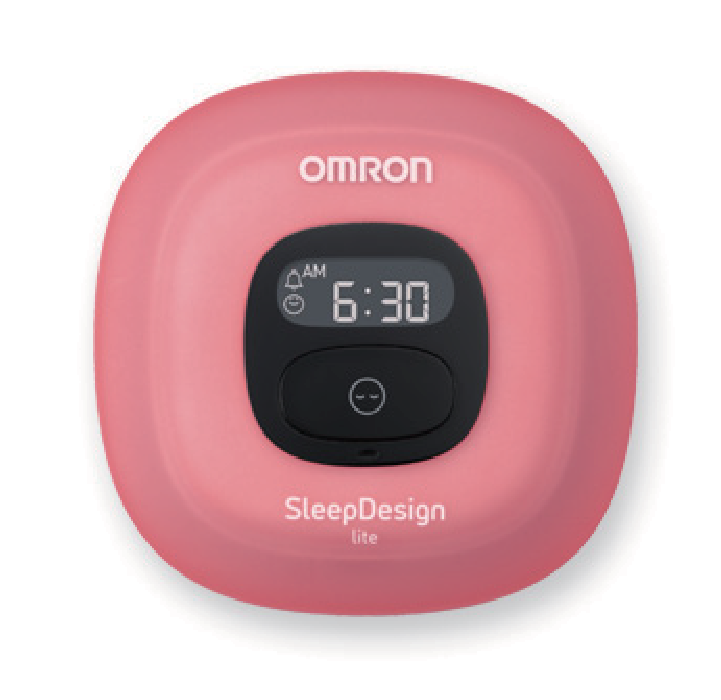
\includegraphics[width=7cm]{eps/omuron.eps}
\caption{オムロン「ねむり時間計」の外観}
\label{omuron}
\end{center}
\end{figure}

neuroonは睡眠サイクルの改善、光セラピーのためのウェラブルマスクである。脳波、眼球の動き、心拍数、血液中の酸素量、加速度、体動と体温全てのセンサーが搭載されている\cite{neuroon}。Delta波やTheta波などを読み取る脳波センサーが備わっているため睡眠サイクルの観測が比較的正確にトラッキングできるのが特徴である。
%\item 正確性:商業目的の製品のため詳しいデーターは明かされていない
%\item 値段:36478円

Zeroは睡眠時無呼吸症候群の解決などを目的としたウェラブルデバイスである \cite{beWellApp}。脳波センサーにより睡眠の各ステージのセンシングが正確にとれるのが特徴であるが、頭に装着しなければならないデバイスなため汗をかきやすく、ユーザの負担になるので長期的な利用に不向きである。\\
iSleepは健康向上のために睡眠時間とその質を観測するスマートフォンのアプリである\cite{iSleep}。スマートフォンに備わっている音声録音機能で咳、いびきや寝言などを記録、加速度センサーで体動を観測し睡眠の質をビジュアル化してユーザに提示する。開発者の Tian は7人の被験者に51日間の実験を遂行し、90\%の正確性で睡眠中のユーザの行動を観測できたと通称している。アプリをダウンロードするだけで簡単に使えるがこと特徴であり、ローンチ10日間で100人のユーザから睡眠に関する詳細なデータを集めている。\\
%\item 値段:361円
%\item 正確性:被験者7人51日間の睡眠で90\%の正確性
BeWellAppもうつ病、心配性、不眠症、高血圧になりにくい生活習慣へ導くために睡眠の長さを測るスマートフォンのアプリである。ユーザによるインプットは一切必要なく、ユーザの充電、加速度からスマートフォン利用頻度・時間を測定、静けさ、部屋の明るさなどから、睡眠スタイルを検知する仕組みになっている\cite{beWellApp}。アプリという形で多くの人に実験をしてもらえる、ユーザは普段の生活となんら変わりなく、過ごせるため、負担がかからないのが特徴である。\\
%\item 効果:8人の被験者に、Jawbone、Zeoと、BESモデルのアプリを試してもらい、全ての人がユーザ体験を過ごせたと結果がきた。
%\item 正確性:睡眠時間+-42分
%\item 値段:商業用目的ではないため不明
以上の先行研究を踏まえると、睡眠の観測の仕方は様々であるということがわかる。最も正確であるとされているのは眼球の動きをトラッキングする手法と脳波センサーであるが、これらは装着型のセンサーのためユーザの負担になってしまう。またデバイスを購入するためのコストがかかってしまう。次に正確なものは体動検知のために使われる電波センサーであるがこれもデバイスの購入を必要とする。よって、ユーザの負担ならずに90\%の正確性も証明されているiSleepをはじめとするスマートフォンアプリケーションが、本研究では睡眠観測の手段としてもっとも適していると判断した。そこで本研究ではiSleepで紹介されているアルゴリズムを参考にしたプログラムを製作した。

\subsection{睡眠時の刺激提示}
 外的刺激を与えることで睡眠に影響を与えようとした研究や製品開発はいくつかの先行研究がある。首都大学の長塚麻美らによる研究では睡眠深度に即した光の刺激を与える抱き枕型のインタフェースを提案している\cite{sleepSheep}。寝付きやすくするために赤に近い黄色の光を点灯させ、波の音を再生するというシステムであるがその実験結果は明らかにされていない。\\
 株式会社タカラトミーが開発した夢見工房は、音や香り、視覚的情報により夢をより理想的なものに近づけるデバイスである。具体的にはユーザが寝る前に「恋愛」、「勇気」や、「冒険」からみたい夢のテーマを選び、睡眠時にそれに紐ずいた音楽と香りが発生する。またボイスレコーダー機能もついており、みたい夢を暗示する声が目覚めない程度の小さな音量で自動的にリピート再生させることもできる \cite{takaratomi}。このように多くの機能が備わっており、気分転換や充実した楽しい時間を作り出すことを目的としているが、その効果を示す実験結果は発表されていない。また香りや音声の種類に限りがあることや香り機械自体の騒音が問題としてあげられており、また値段も14,800円と高めである。\\
\begin{figure}[htbp]
\begin{center}
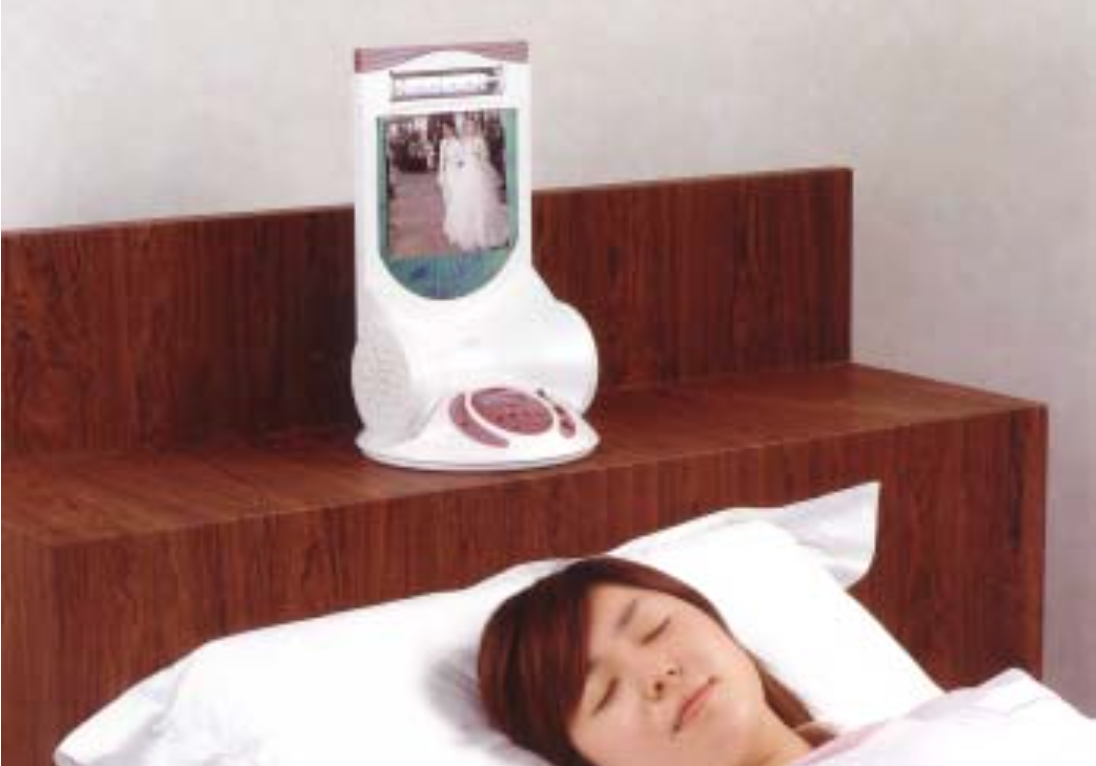
\includegraphics[width=14cm]{eps/takaratomi.eps}
\caption{夢見工房}
\label{takaratomi}
\end{center}
\end{figure}
 他にも明晰夢を促進するためのツールとしてiWinksにより開発されたAURORAがある\cite{iWinks}。これはレム睡眠時に光による刺激を与えることで、ユーザに夢を見始るという信号を送って明晰夢を促すデバイスである。脳波センサー(EEGセンサー)と加速度センサーが組み込まれており、睡眠の質の観測においてはクリニックにより検証されたものであるとウェブページ上には書かれている。しかし明晰夢への効果に関する実験結果が明らかにされておらず、また値段も3,6000円と非常に高額である。\\
 本研究の提案と非常に近しいスマートフォンアプリとして2012年のEdinburgh International Science Festivalを機にローンチされたDreamOnがある。睡眠中に音楽を流すことで夢の内容に影響を与えるアプリである。多くユーザに夢の研究に参加してもらい音が夢に影響を与える否か、国籍や年齢によって結果に違いが現れるかについて明らかにすることを目的としている。App Storeでユーザによる評価は385人によってレーティングが行われており、評価は5点中3である。下記の図\ref{DreamOnMusicSlection}はDreamOnの音を選択画面である。Press Packは自分が注目の元となる夢、Relaxing Rainforestは森林の中で鳥やコオロギの鳴き声を聞きながらリラックスできる夢、Ocean Veiwは海でリラックスする夢、Travel the Worldは自転車、電車、船や飛行機に乗って世界中を旅する夢など、合計30個の夢の中から自分の見たい夢を選択できるようになっている。
\begin{figure}[htbp]
 \begin{minipage}{0.45\hsize}
  \begin{center}
   \includegraphics[height=90mm]{eps/deamOnMusic.eps}
  \end{center}
  \caption{DreamOn音選択画面}
  \label{DreamOnMusicSlection}
 \end{minipage}
 \begin{minipage}{0.45\hsize}
  \begin{center}
   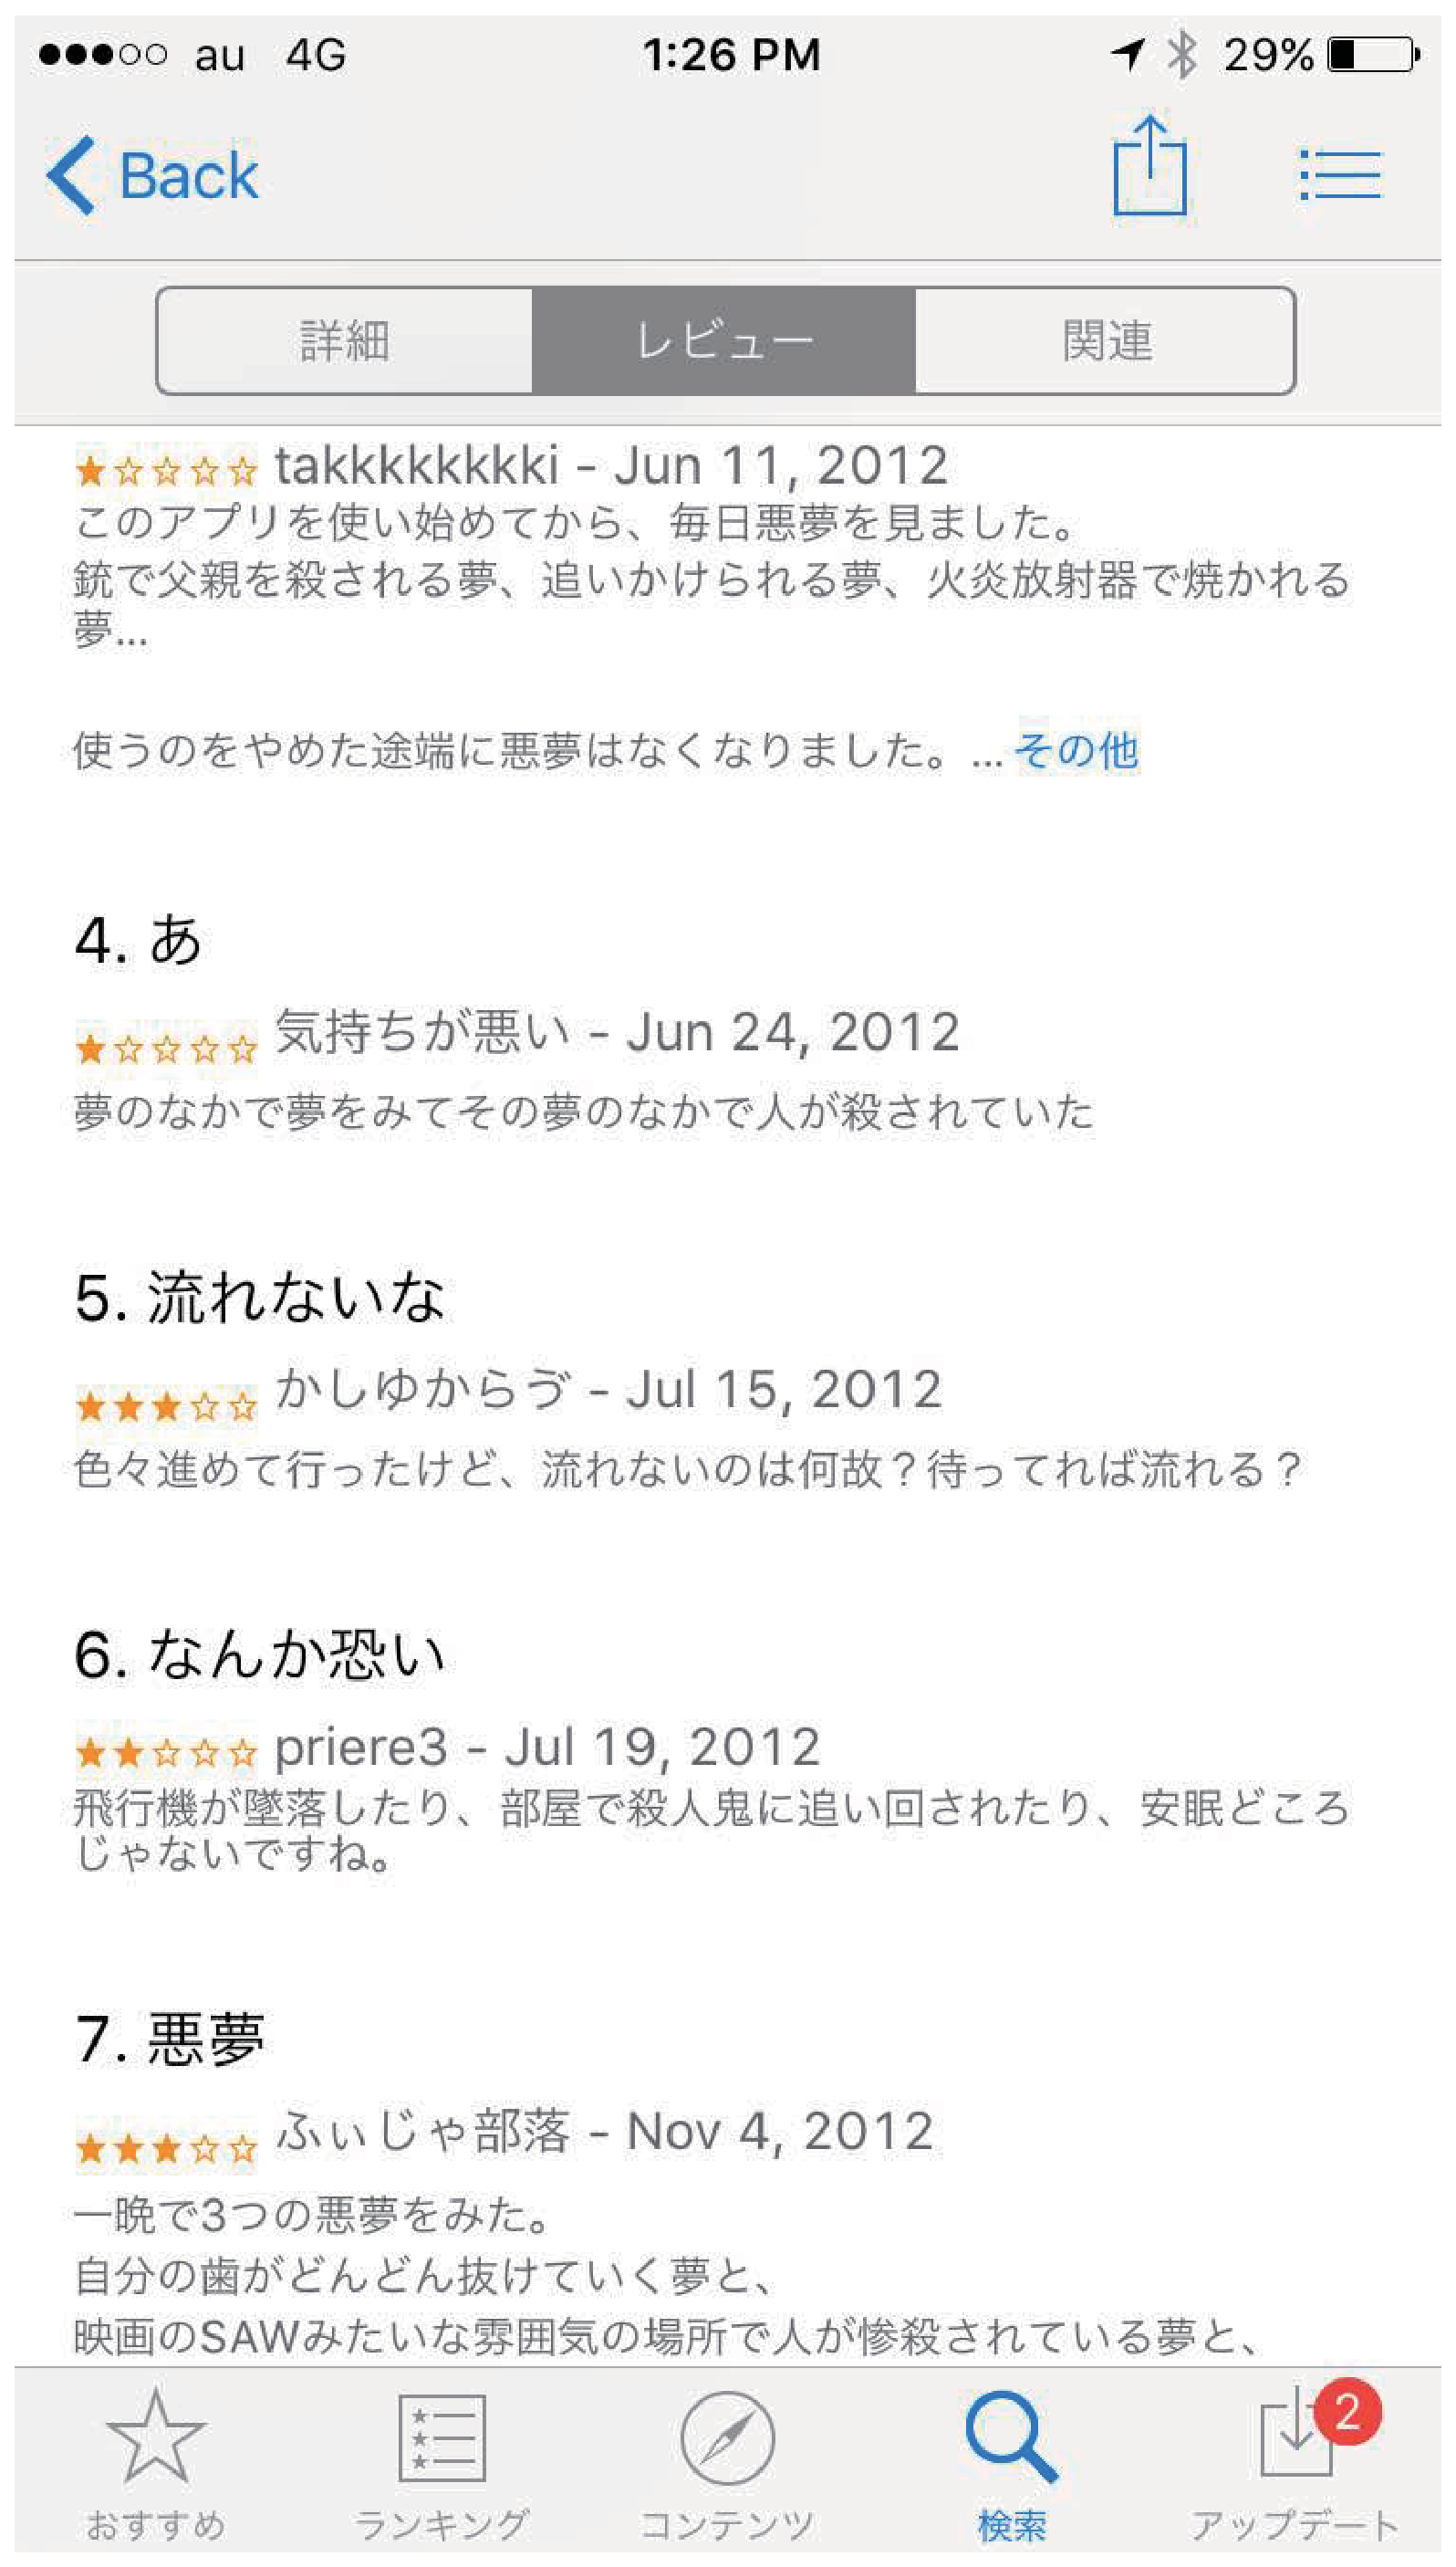
\includegraphics[height=90mm]{eps/dreamOn.eps}
  \end{center}
  \caption{DreamOnのユーザレビュー}
  \label{DreamOnImage}
 \end{minipage}
\end{figure}
集められたデータの数は13万件だと公式ウェブサイトに書かれているが、具体的な実験結果は未だ投稿されていない。そこでApp Storeのユーザレビューを代わりに図\ref{DreamOnImage}に示した。悪夢を見たなどの不満を訴えるレビューが多く見受けられた。音を流すタイミングについては説明がなかった。\\
他にも「見たいユメをみせてくれるかもしれないアプリケーション」と説明がされているユメミール \cite{yumemiru}というアプリがある。このアプリには森を散歩するユメ、海へ行くユメ、空を飛ぶユメ、告白されるユメ、お金持ちになれるユメ、初夢用富士山の夢、合格する夢の7つの選択肢がある。App Storeのユーザレビューを見るとそもそも音が鳴らないなど機能面での不具合があることがわかる。音の流し方やタイミングについては説明がなかった。
\begin{figure}[htbp]
 \begin{minipage}{0.45\hsize}
\begin{center}
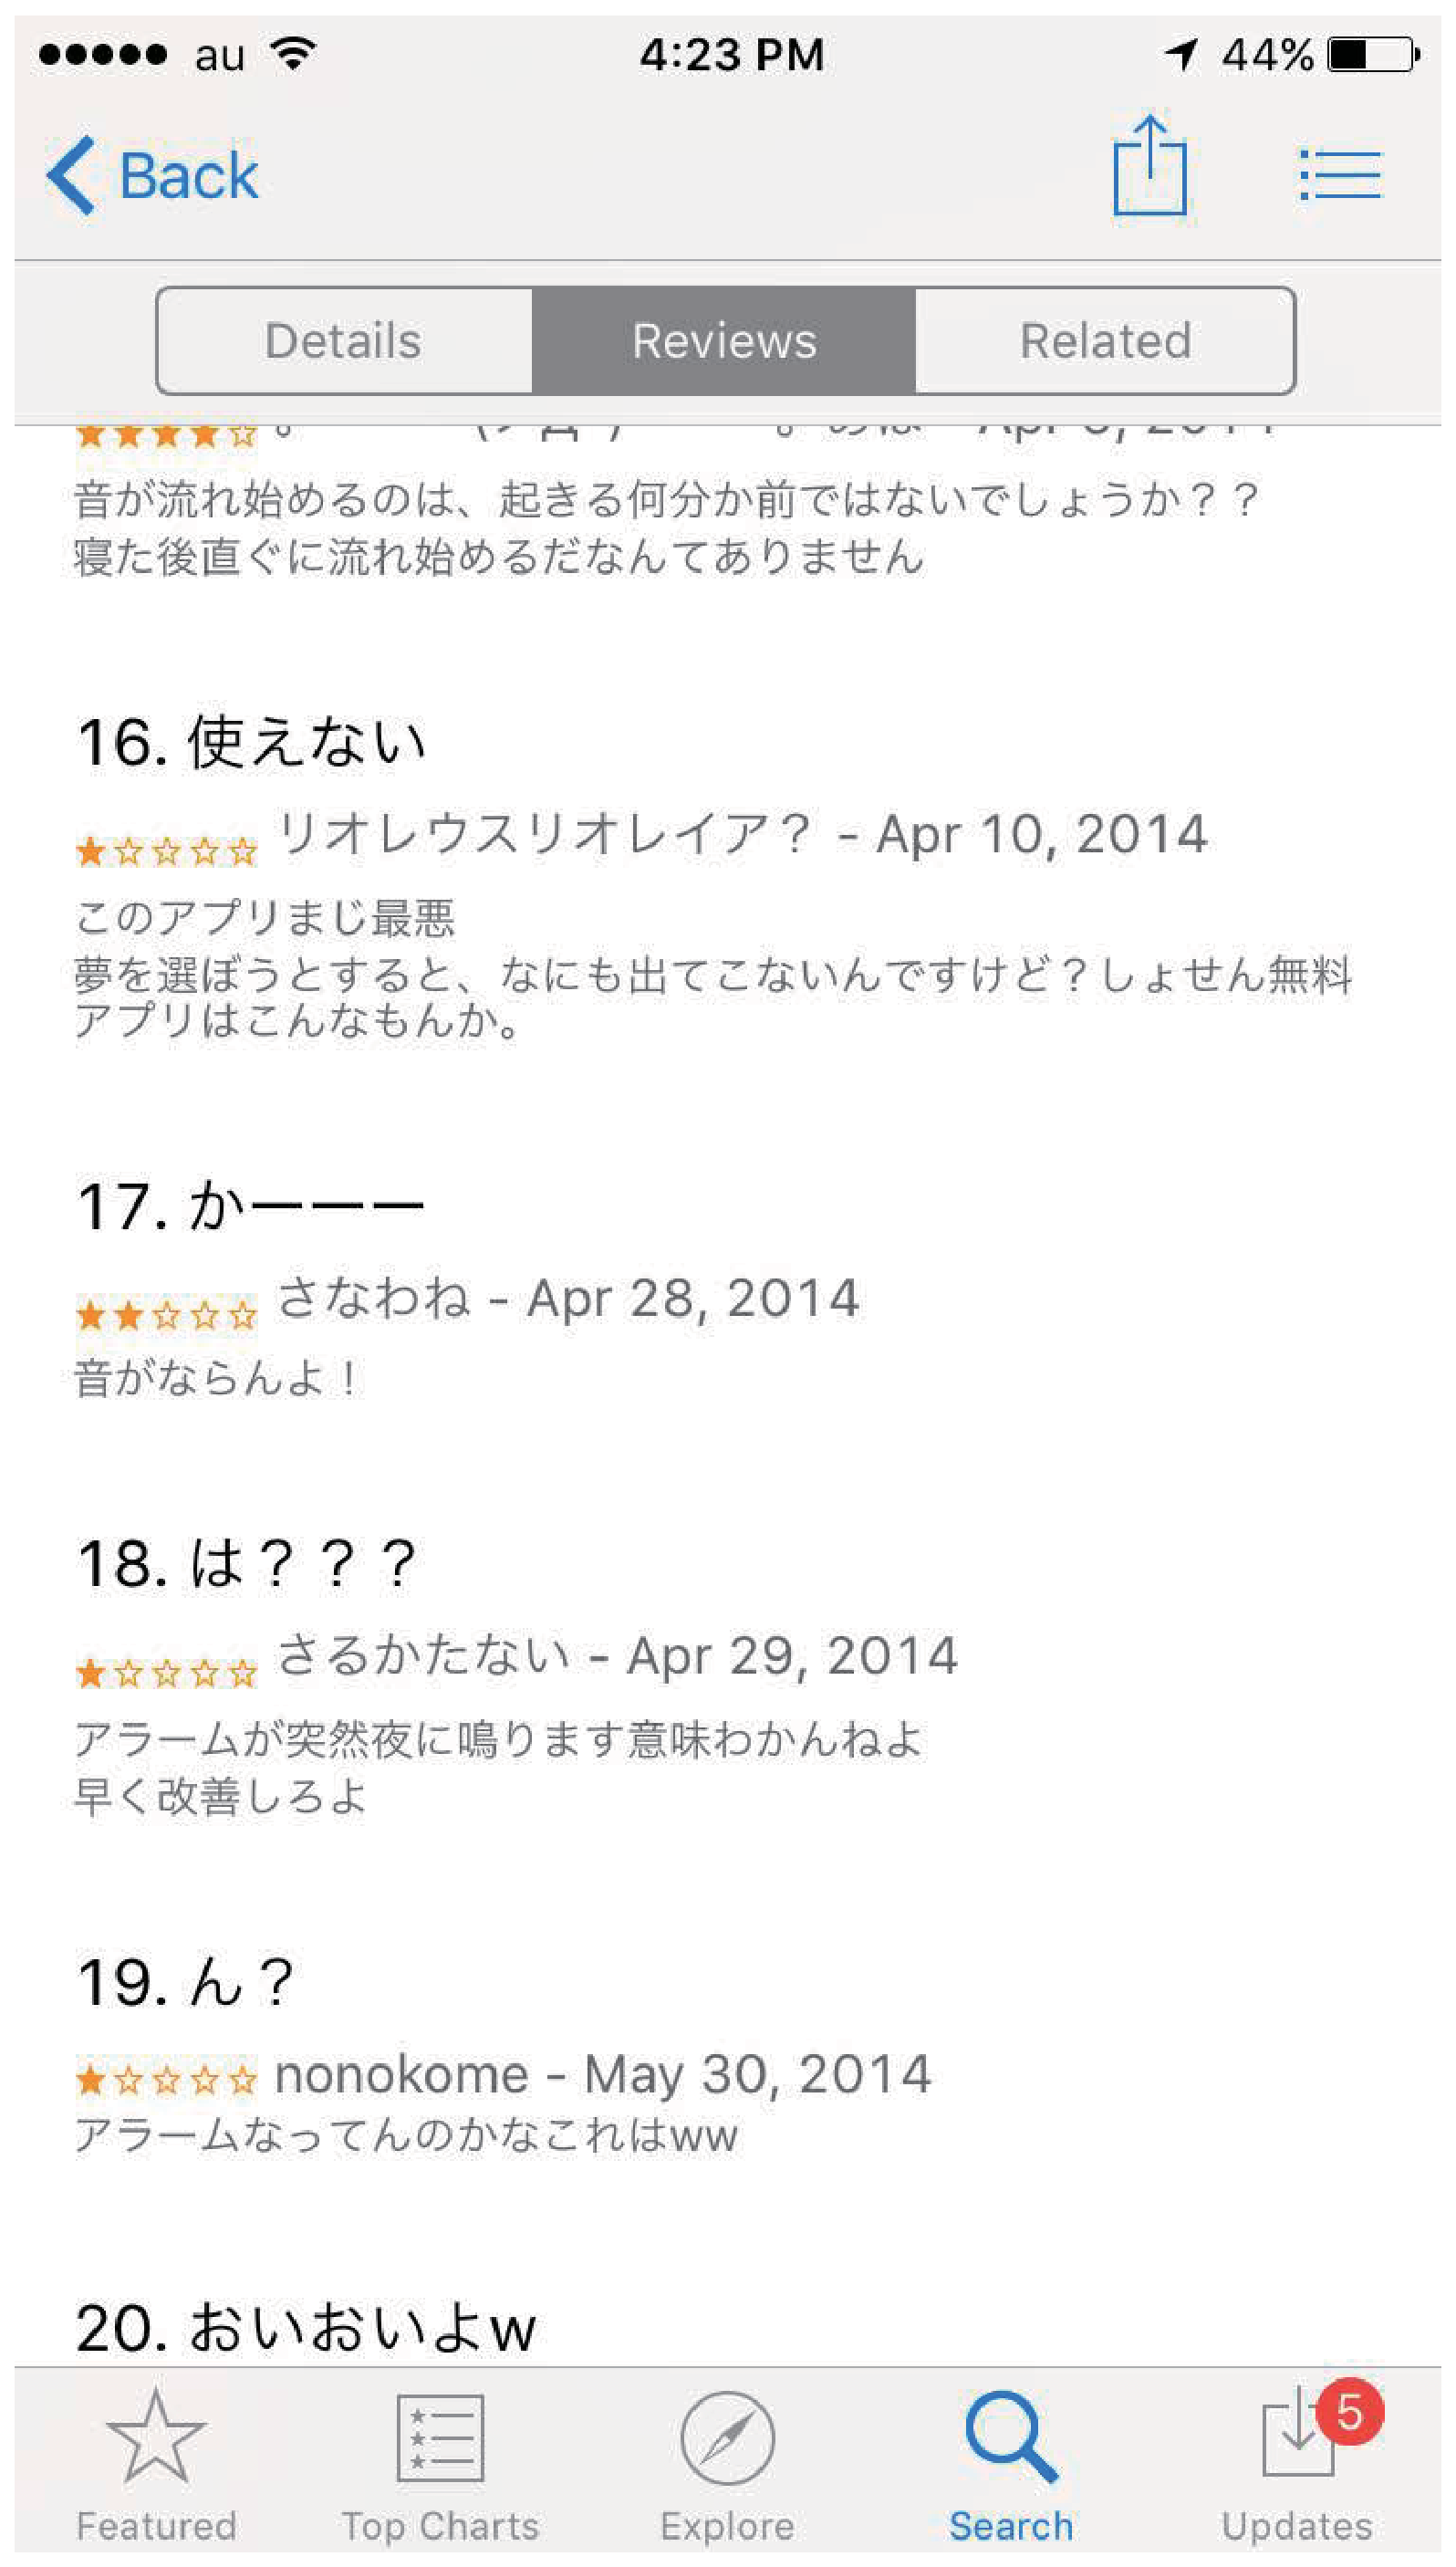
\includegraphics[height=90mm]{eps/yumemiru.eps}
\caption{ユメミールのユーザレビュー}
\label{DreamOnImage}
\end{center}
\end{minipage}
\end{figure}

\section{本研究の位置付け}
Head Mounted Display(HMD)は仮想現実を体験するためにメジャーな手法として注目を浴び開発が進んでいる。しかし体験をするためにはOCULUSを始めとした高価なデバイスを購入しなければならない。3 次元のコンテンツを作成するには技術やコストが高くユーザが望むコンテンツを気軽に作れるようにはなっていない。\\
そこでDreamDateは明晰夢に着目した。明晰夢は睡眠という習慣をより有効に活用し、金銭的コストをかけることなく遂行することができる。1章でも紹介したが明晰夢を体験するためのステップとしてMnemonic Induction of Lucid Dreams (The MILD Technique)がある。しかしThe MILD Technique には労力が必要で誰もが気軽に始められるものとは言い難い。DreamDateはMILDに比べてユーザの負担を下げることを目的に誰も気軽に使い始められるようにスマートフォンアプリでサポートをする。夢を忘れない体質になるためにThe MILD Techniqueのステップの1つとして紹介されている夢日記をアプリの機能に組み込むことにした。またDreamDateのモニタリングシステムは睡眠観測スマートフォンアプリiSleep\cite{iSleep}を参考に構築した。\\
明晰夢を促進するシステムとして株式会社タラトミーによる夢見工房やスマートフォンアプリDreamONやユメミールなどが既に開発されている。しかしどのプロダクトも実験結果に個人差が出て、機能性が証明されていないのが現状である。夢見工房やDreamOnはレム睡眠を検出して睡眠中に刺激を与えることで夢に影響を与えるシステムである。刺激はプロダクトに既に登録されている音や香りからユーザが選べるようになっているものが多い。全ての被験者に同じ音とタイミングで刺激するのではなく、よりユーザの思い通りの夢を見やすいように流す音に一人一人慎重に吟味した上で選定した上で実験を行うことにした。詳細は第3章と第4章で述べる。

DreamDateシステムに求められる要件を以下にまとめる:
\begin{itemize}
\item ユーザ一人一人の要望に合った音を選ぶシステム
\item 明晰夢で仮想現実を体験できる
\item HMDのように高価なデバイスを必要としない
\item MILD Techniqueと違って、負担の少ないユーザ体験
\end{itemize}